%!TEX root=./LIVRO.tex
\captionsetup{font={small, it}}
\captionsetup{justification=raggedright, singlelinecheck=false}

\chapter{Apresentação}

\section{A \textit{Plataforma digital Revisa SAEB}}

% Felipe

A \textit{Plataforma digital Revisa SAEB} foi desenvolvida para alunos 
do 1º ao 9º ano do Ensino Fundamental. Por meio dela, eles
têm acesso às versões digitais ao livro digital, simulados, vídeos e jogos. 

Já os professores, além de terem acesso ao
mesmo conteúdo que os alunos, contam com uma série de vídeos de capacitação 
e  relatórios sobre o desempenho da sua turma.

Os coordenadores, por sua vez, podem consultar  diretamente na plataforma relatórios de frequência e pontuação
com os dados de toda região.


A \textit{Plataforma digital} tem como base um
sistema integrado de gestão de código aberto chamado Odoo, 
que oferece  módulos e recursos para a educação adaptáveis às
necessidades específicas. Vale lembrar que esse mesmo sistema é está sendo usado
em todas as escolas públicas de Portugal desde 2014.\footnote{ Para saber mais sobre o uso do projeto Odoo, consulte 
\href{https://www.odoo.com/pt_BR/partners/thinkopen-solutions-portugal-2614}{Thinkopen Solutions — Portugal.}}
%\url{}




\section{Como acessar?} 

\begin{itemize}
\item URL da \textit{Plataforma Digital Revisa SAEB digital}:  \url{revisasaeb.com.br}.

\item Credenciais do aluno: \textbf{aluno-teste} e senha: \textbf{minhacidade}
\item Credenciais do professor: \textbf{professor-teste} e senha: \textbf{minhacidade}
\item Credenciais do coordenador: \textbf{coordenador-teste} e senha: \textbf
 {minhacidade}\footnote{ Caso tenha alguma dúvida ou dificuldade, favor
 entrar em contato com Elio Viniski pelo email elio@edoo.me ou
 telefone +51 9252-5268 (suporte técnico responsável). }
\end{itemize}

\section{Quais são as áreas principais da plataforma?}

Após o \textit{login}, professor e gestores terão acesso a duas áreas: uma chamada \textit{frontend}, 
dedicada totalment aos cursos, e outra chada de \textit{backend}, voltada para a leitura de relatórios
e proposta de eventos. Para acessar o backend, é necessário clicar no ícone indicado na foto abaixo:
\medskip


\noindent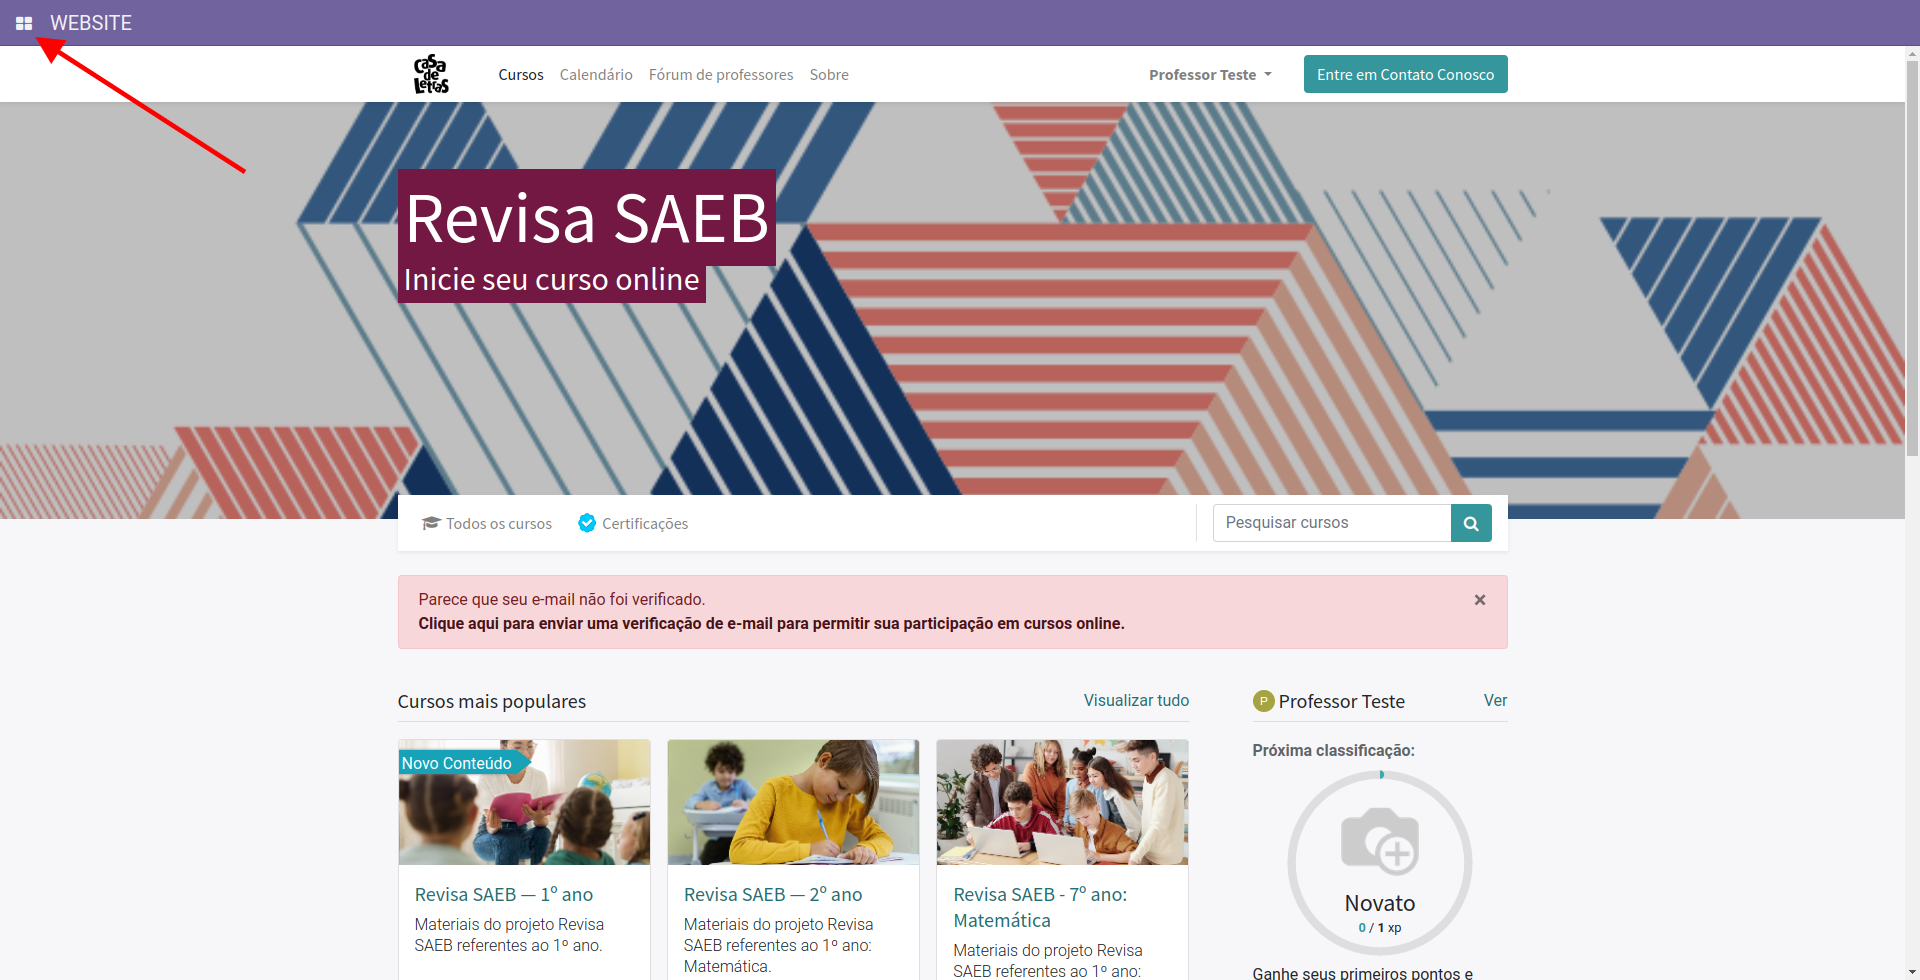
\includegraphics[width=\textwidth]{imgs/backend.png}\medskip

No \textit{frontend} estão os cursos e um fórum, de acesso restrito.
No \textit{backend} estão os relatórios dos simulados e treinos e a área de 
convocação de eventos, que podem servir para disparos de emails e SMSs.
Veja abaixo:\medskip

\noindent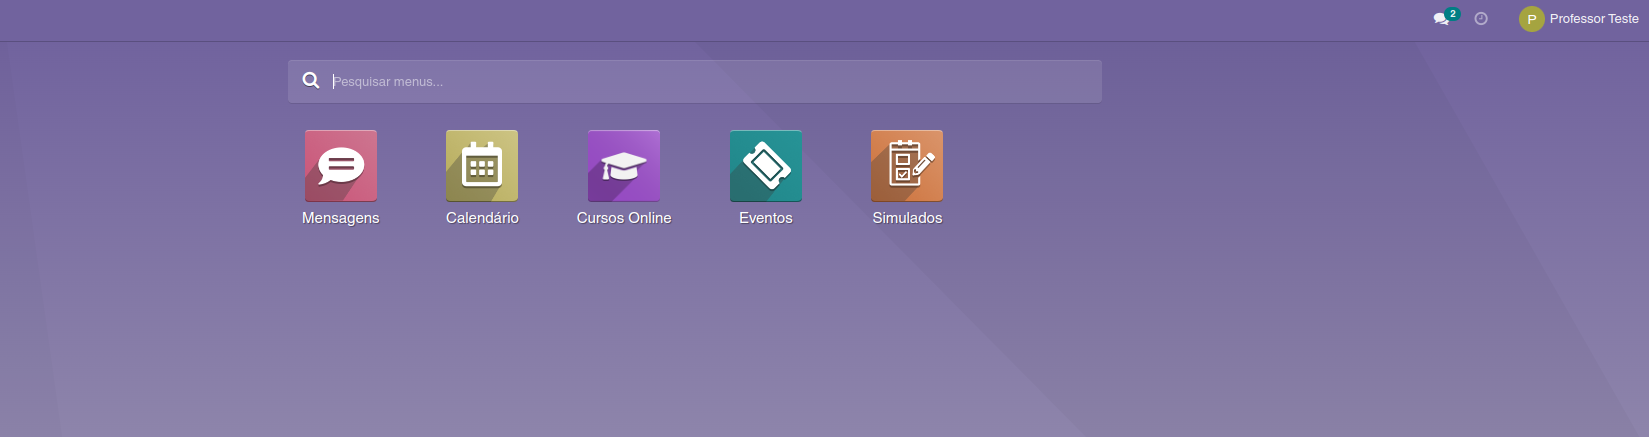
\includegraphics[width=\textwidth]{imgs/backend_home.png}\medskip


Para o aluno serão oferecidos os curso do seu ano, divididos em seções, e o calendário de eventos.

O perfil do coordenator é muito semelhante ao de professor, mas somente ele tem acesso
aos dados das escolas do município de maneira consolidada. Fazem parte desses dados  afrequência, notas e
certicações dos alunos e o grau de acertividade das questões.


\section{Diferenciais da \textit{Plataforma}}

\begin{figure}[h]
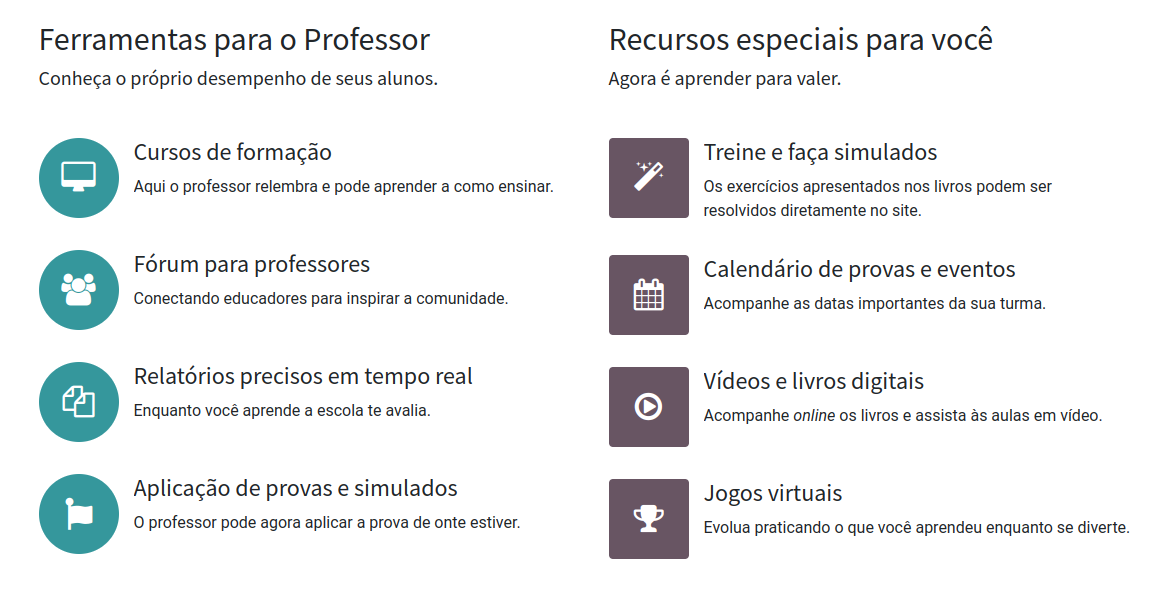
\includegraphics[width=\textwidth]{imgs/sobre}
\end{figure}

Acima são mencionadas algumas das principais características presentes na \textit{plataforma}.
Cabe destacar ainda as funcionalidades de \textit{gamificação}, que
definem roteiros e avatares a serem conquistados com a 
pontuação do aluno. 

\begin{figure}[b]
\centering 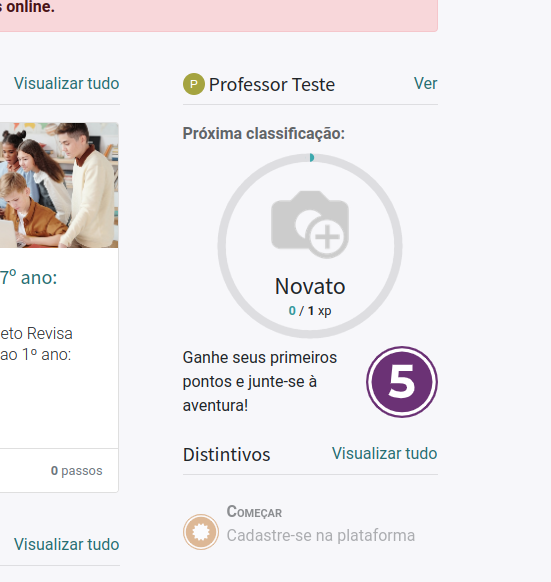
\includegraphics[width=0.4\textwidth]{imgs/game}
\end{figure}




\chapter{Imagens do site}

\mbox{}

\begin{figure}[h]
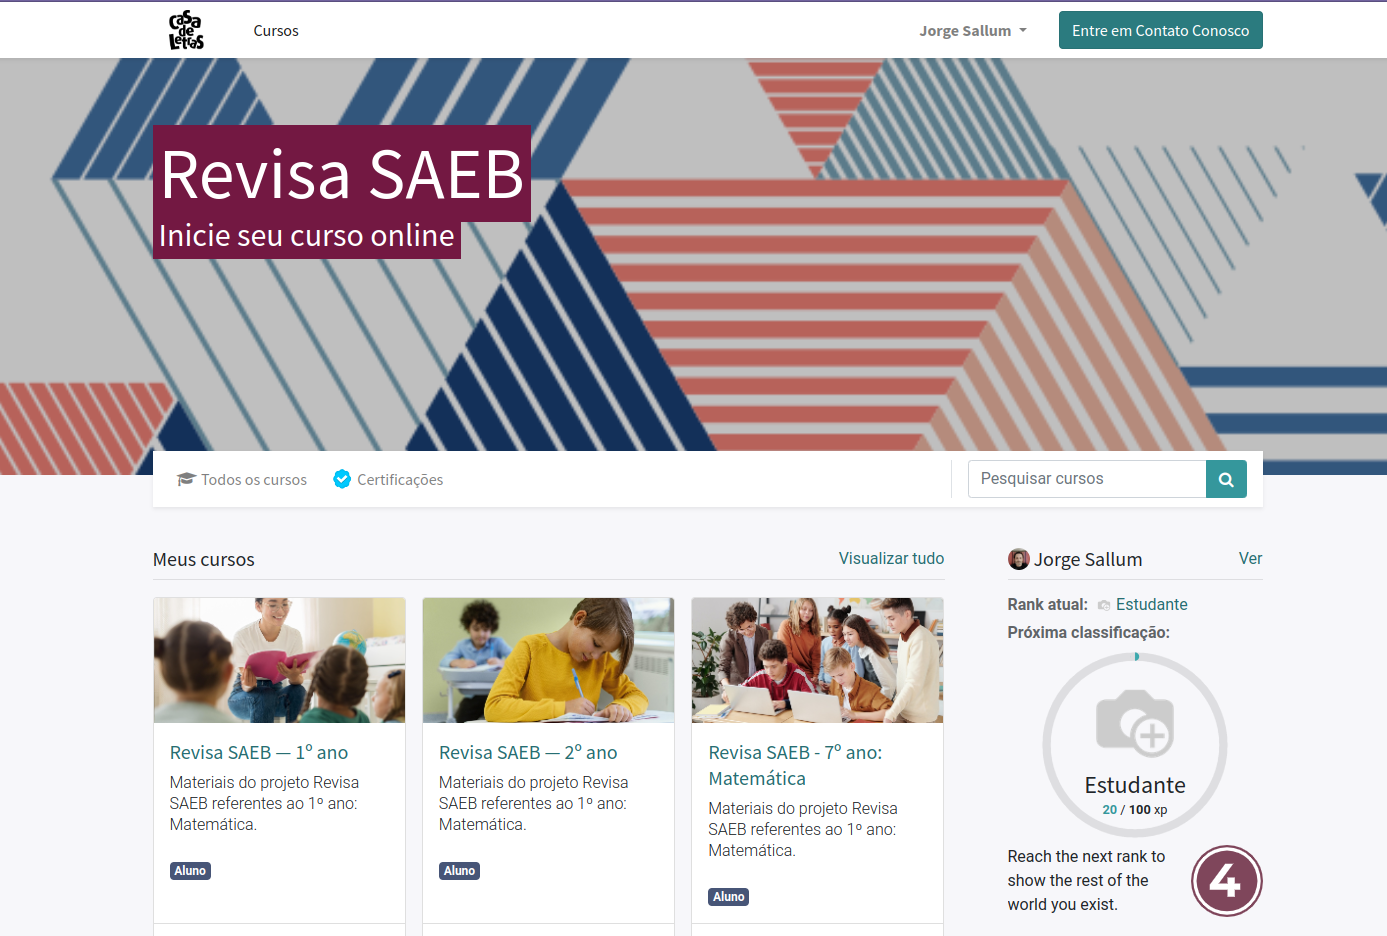
\includegraphics[width=\textwidth]{imgs/front}
\caption{Home da Plataforma}
\end{figure}

% \begin{figure}
% 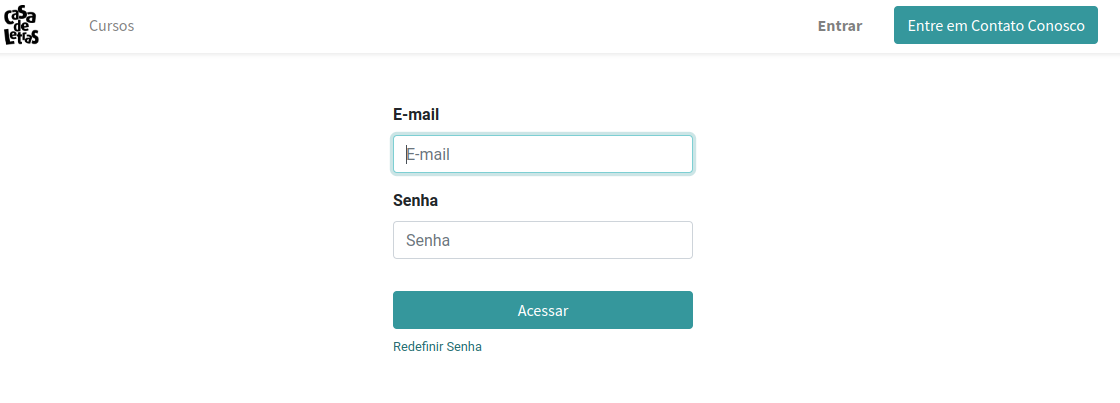
\includegraphics[width=\textwidth]{imgs/login}
% \caption{Tela de login}
% \end{figure}


\begin{figure}[H]
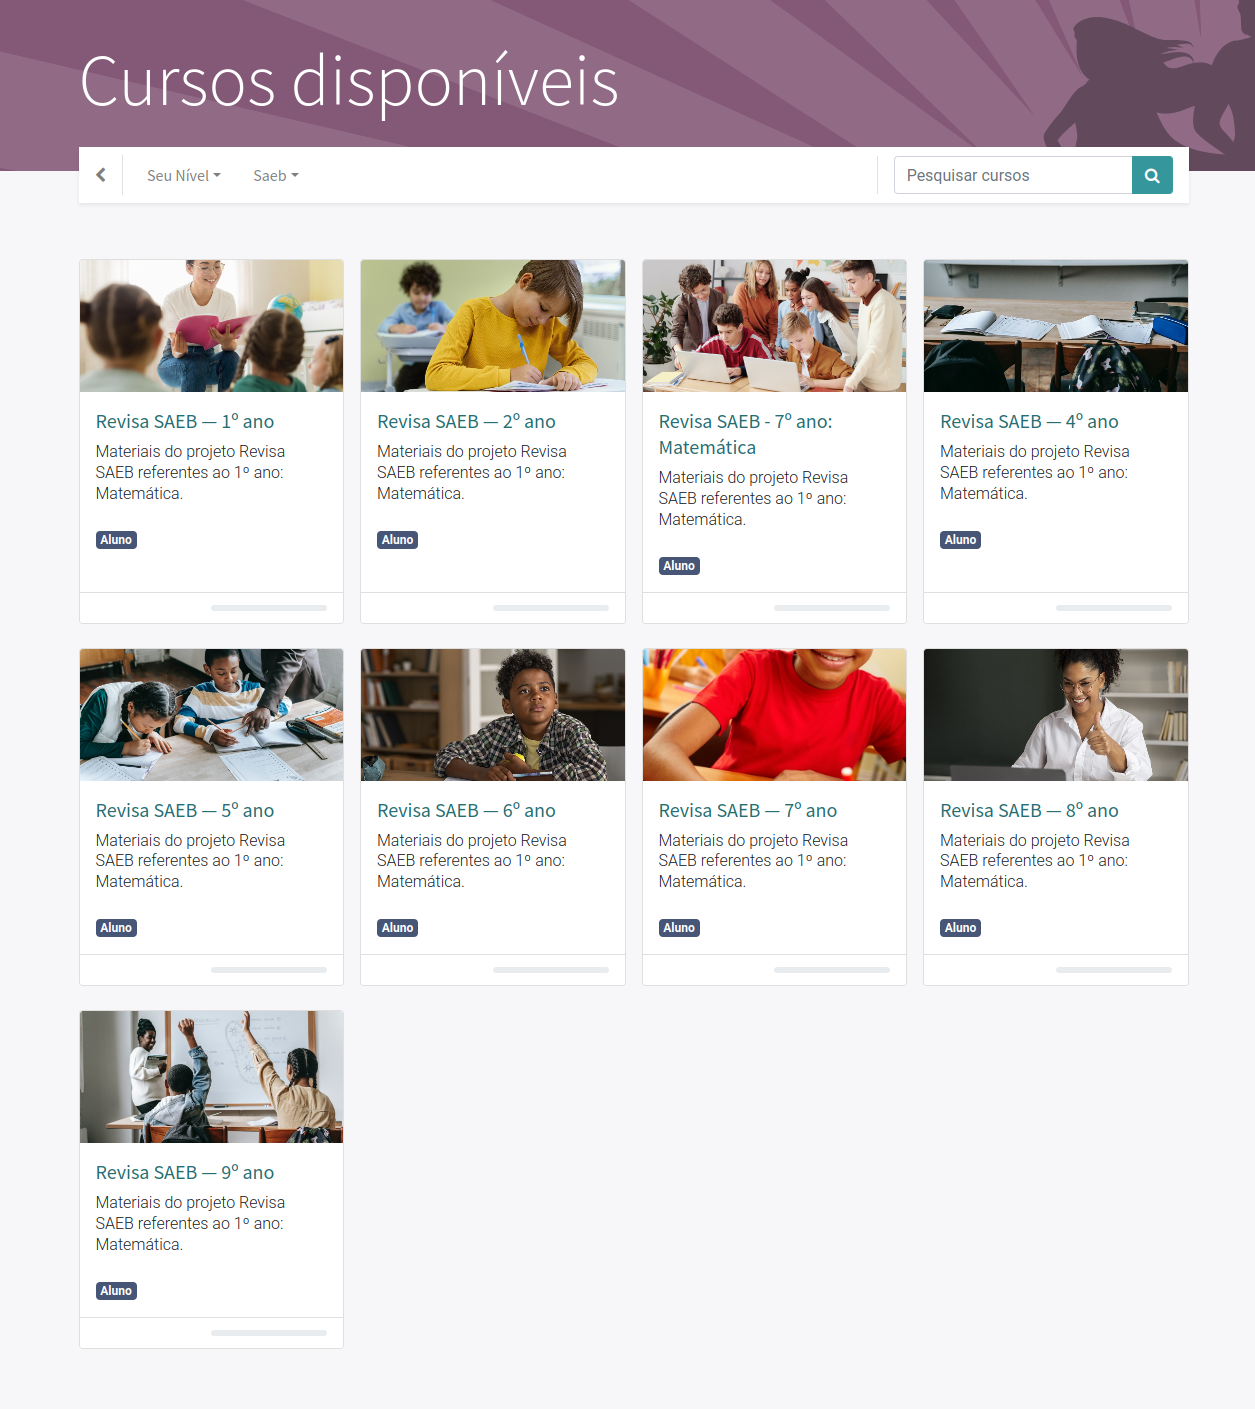
\includegraphics[width=\textwidth]{imgs/cursos}
\caption{Todos os cursos do aluno divididos por ano}
\end{figure}


\begin{figure}[H]
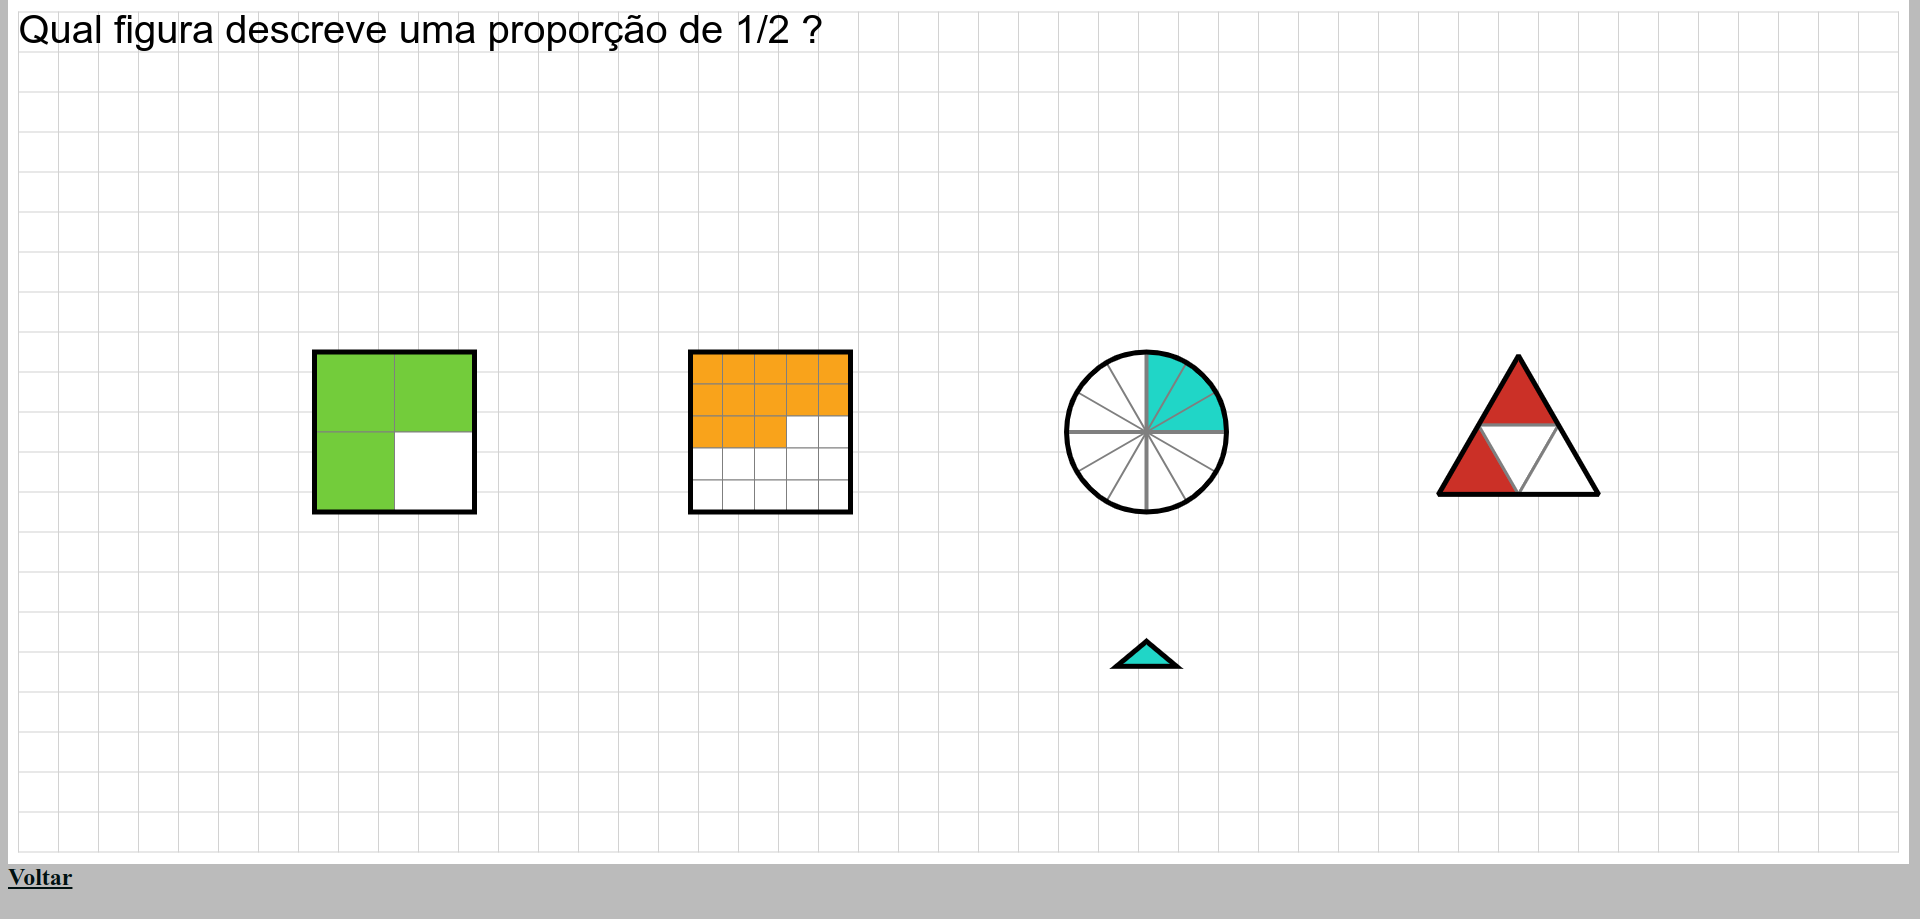
\includegraphics[width=\textwidth]{imgs/jogo1}
\caption{Jogo sobre frações}
\end{figure}


\begin{figure}[H]
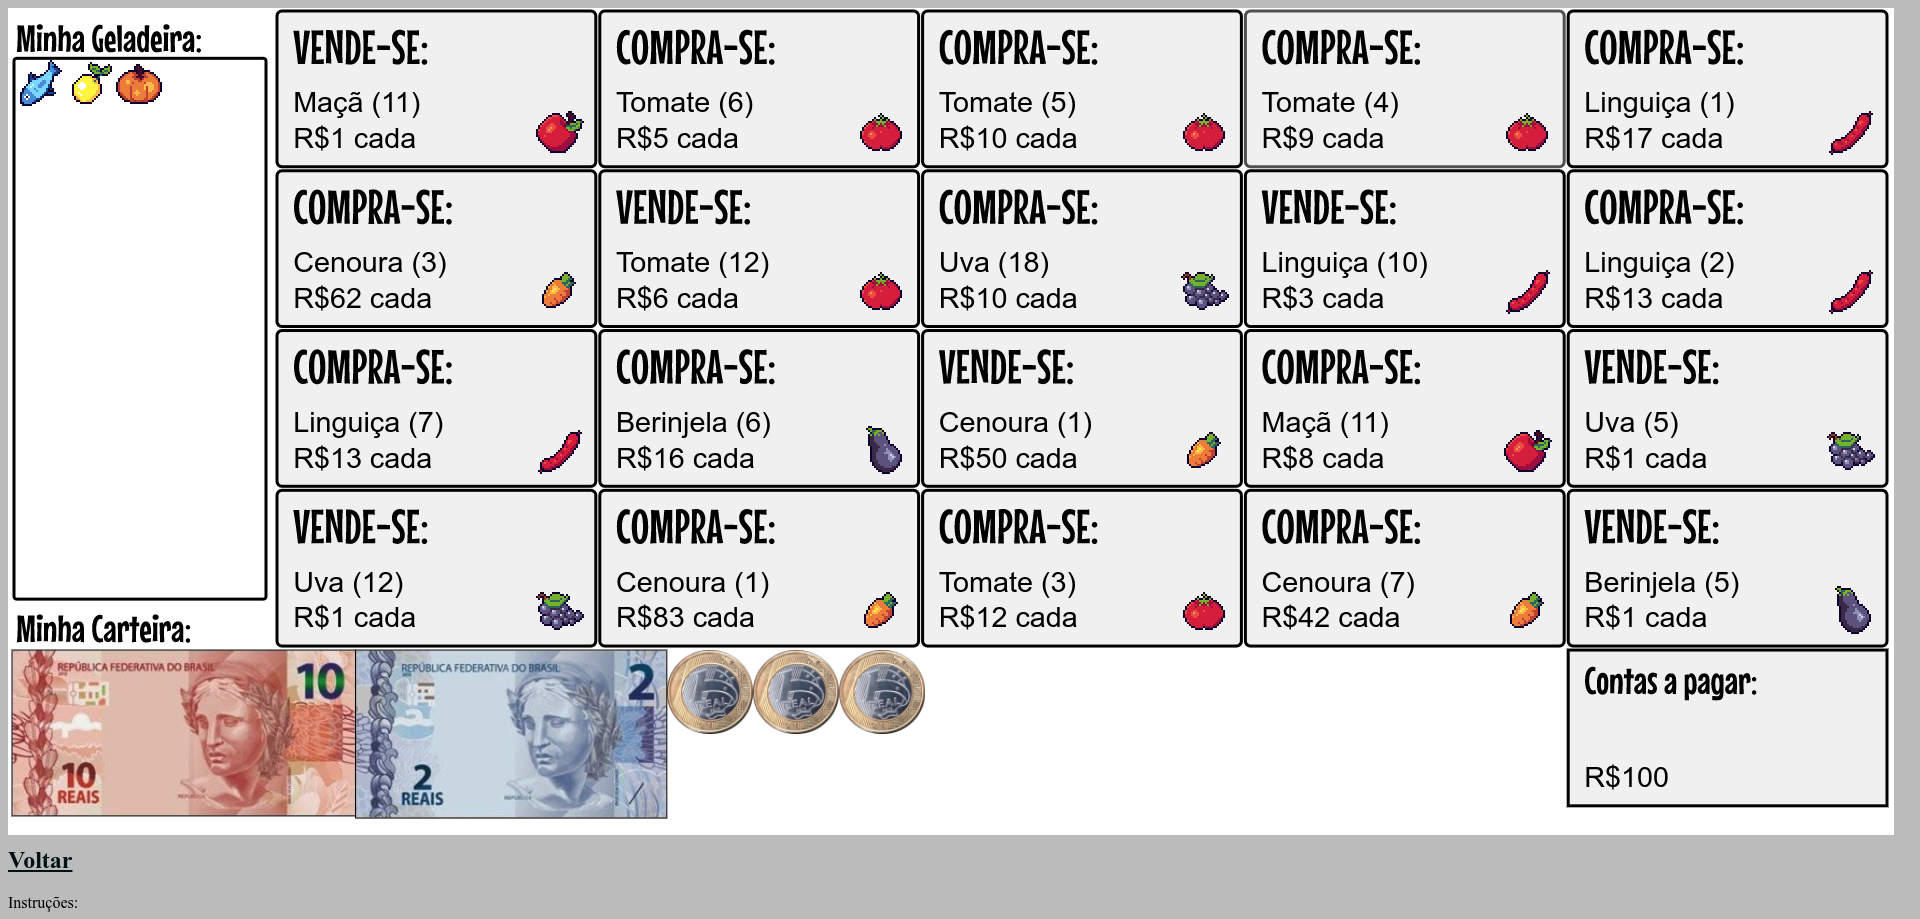
\includegraphics[width=\textwidth]{imgs/jogo2}
\caption{Jogo sobre uso de dinheiro}
\end{figure}


\begin{figure}[H]
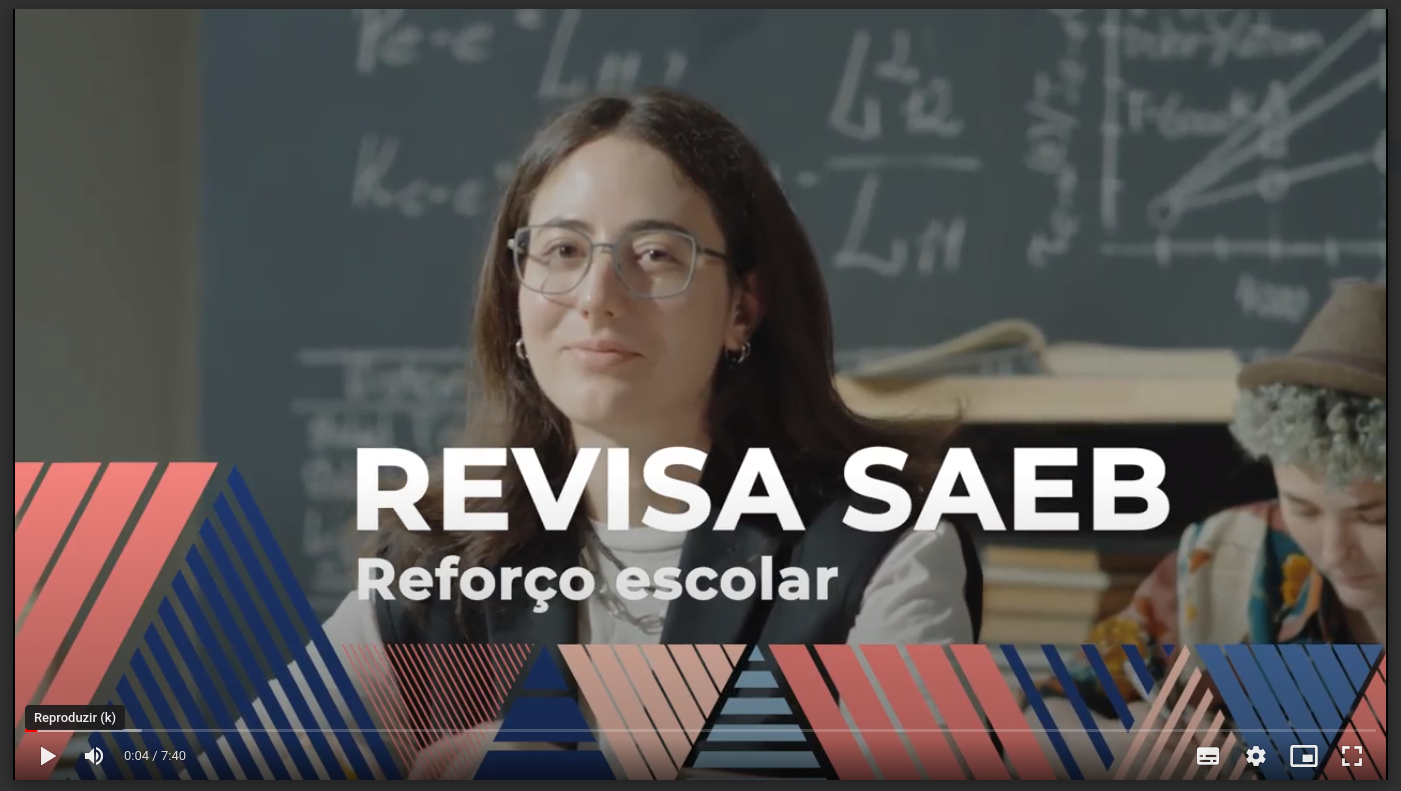
\includegraphics[width=\textwidth]{imgs/video1}\bigskip

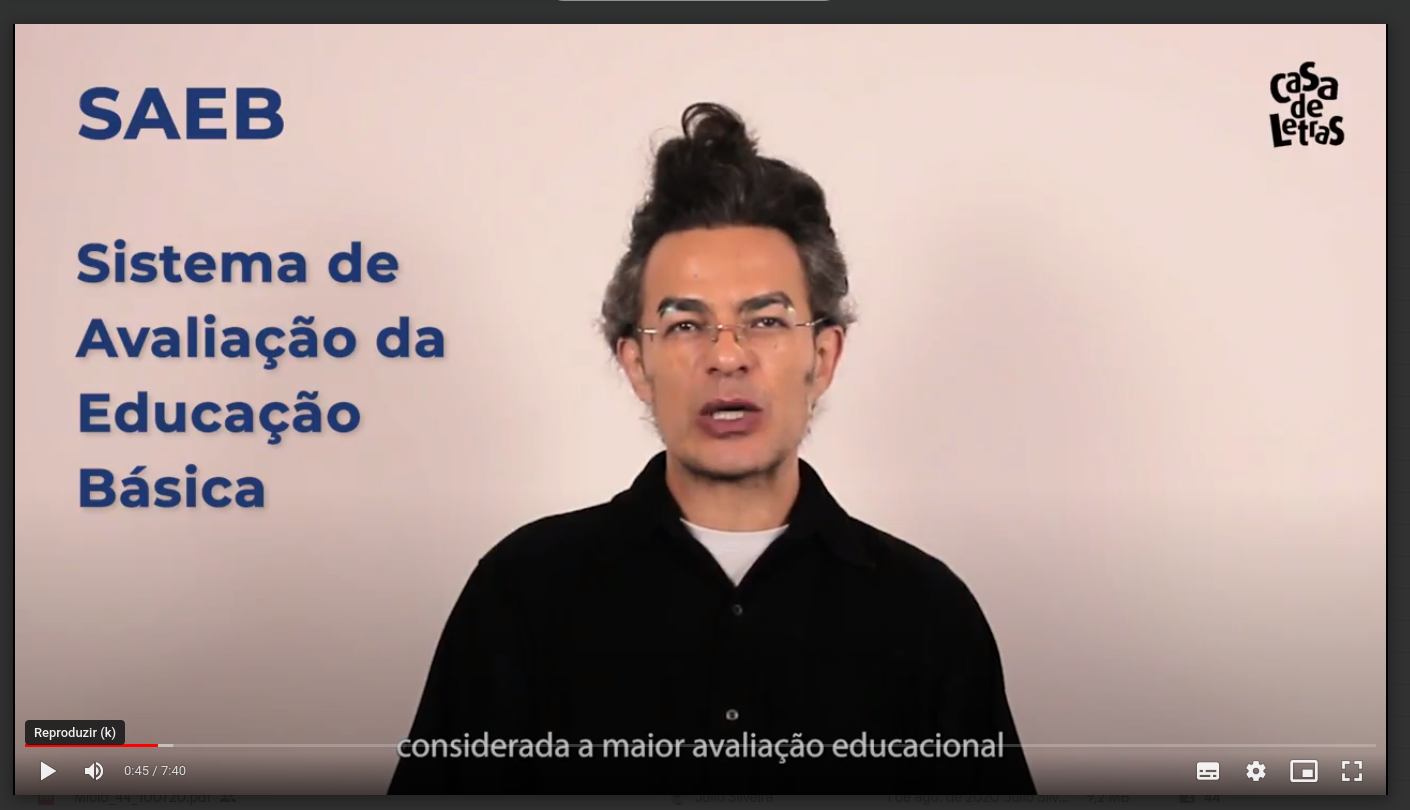
\includegraphics[width=\textwidth]{imgs/video-2}
\caption{Vídeos}
\end{figure}



\begin{figure}[H]
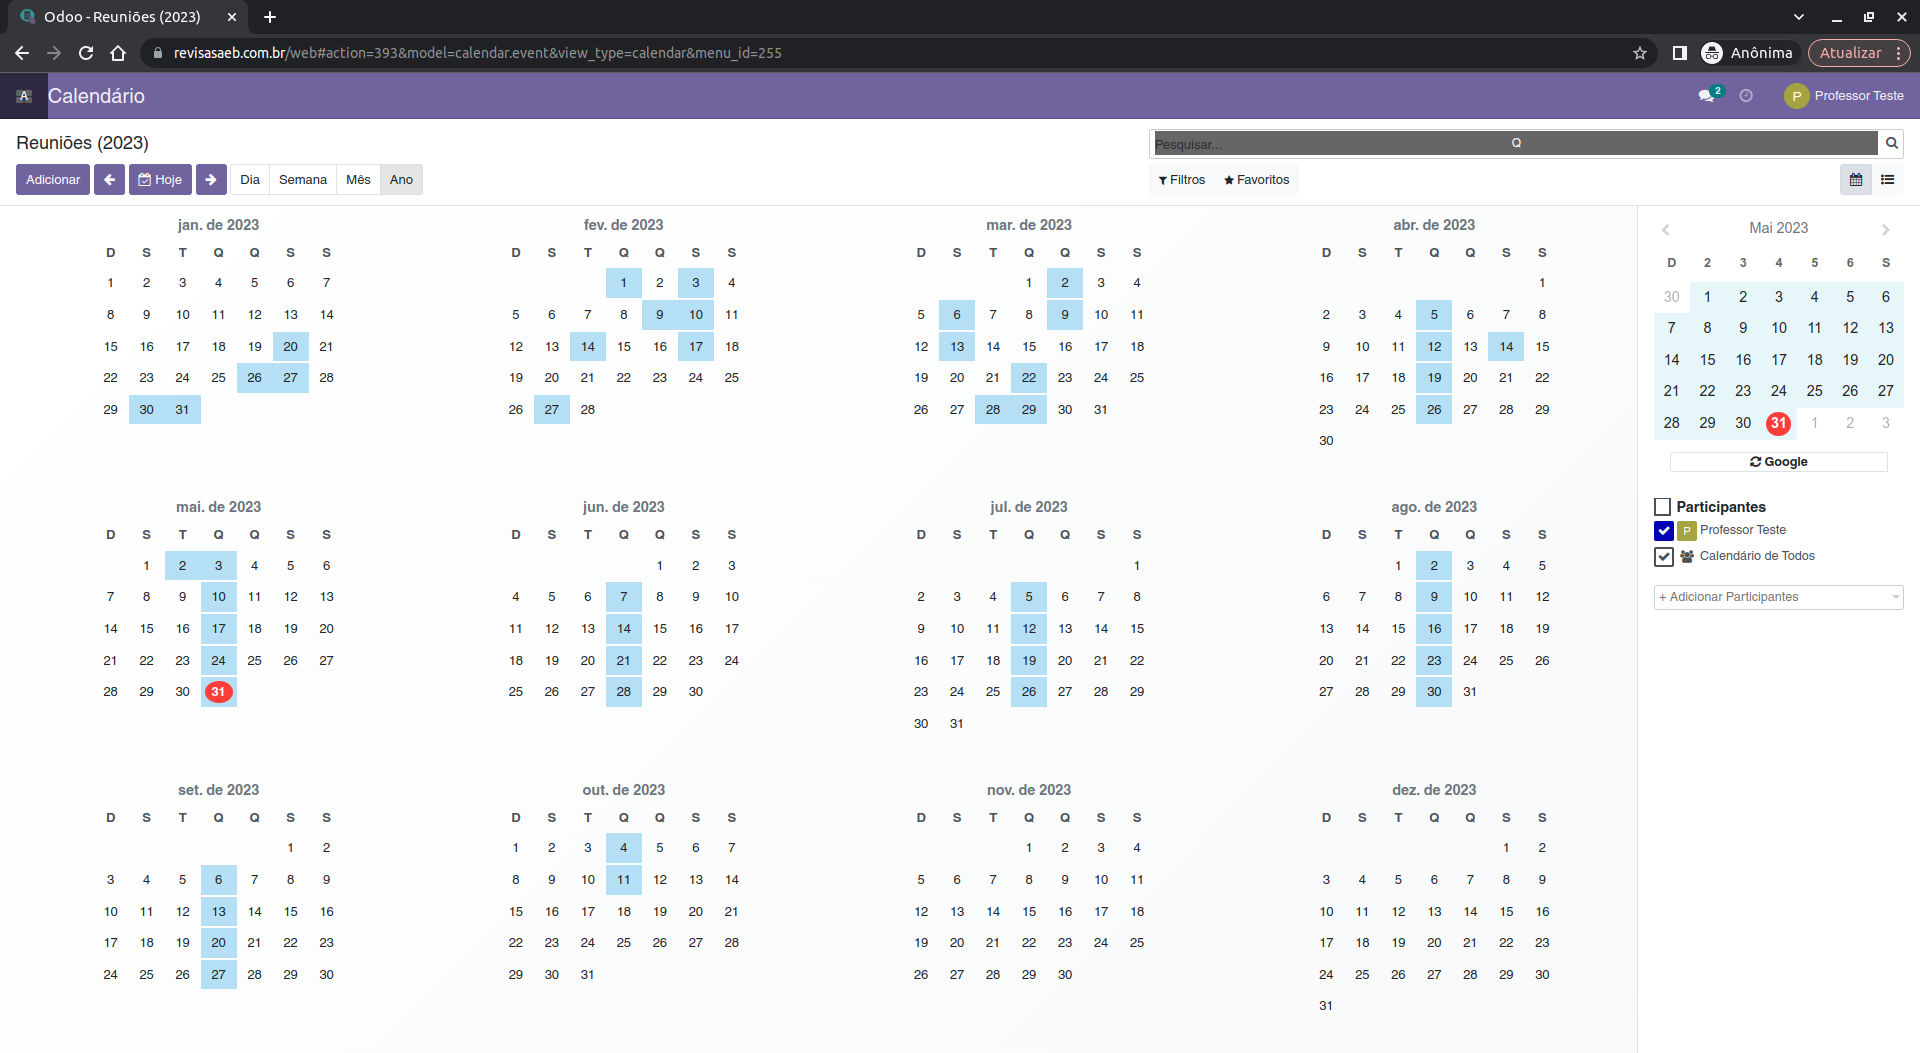
\includegraphics[width=\textwidth]{imgs/calendario}
\caption{Calendário de administração de eventos}
\end{figure}


\begin{figure}[H]
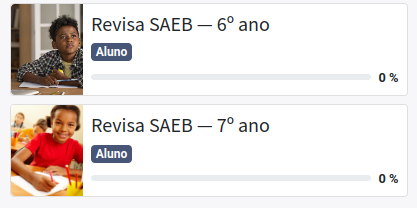
\includegraphics[width=\textwidth]{imgs/progresso}
\caption{No perfil do aluno é possível ver o progresso de cada curso}
\end{figure}

\begin{figure}[H]
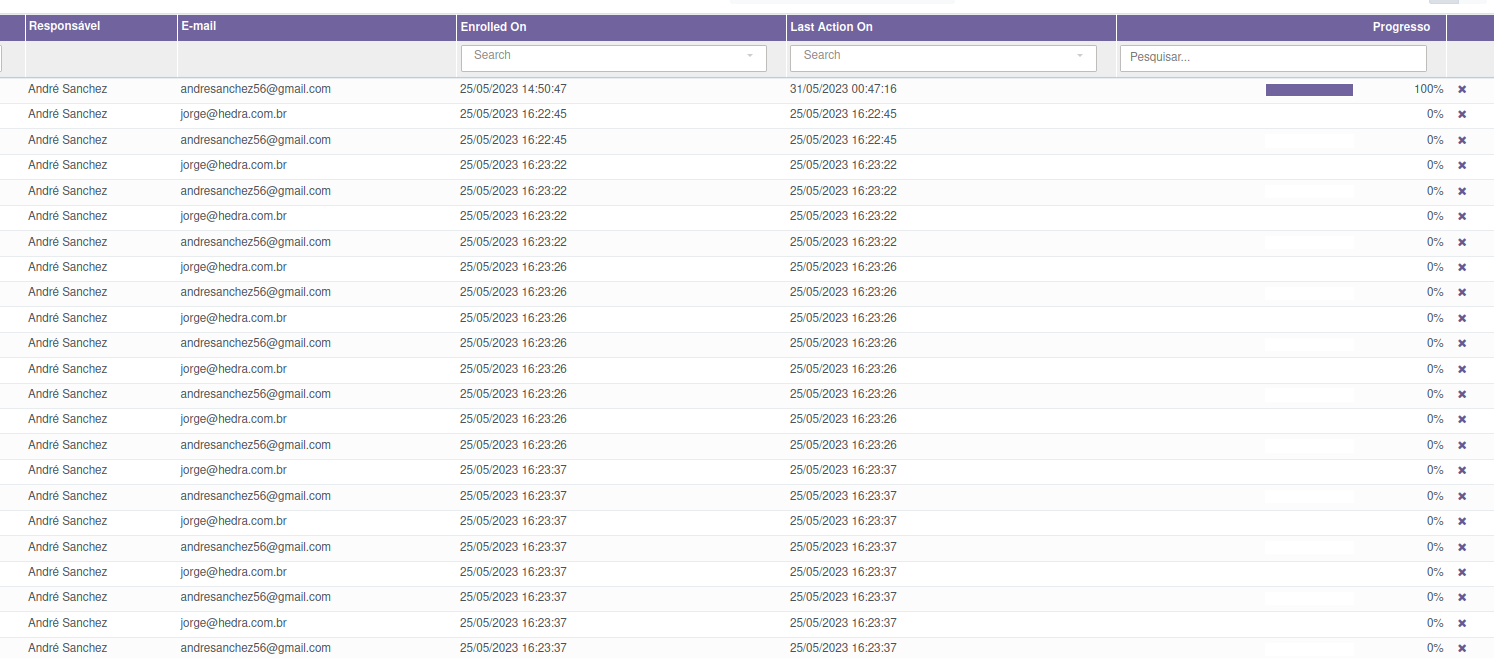
\includegraphics[width=\textwidth]{imgs/relatorio}
\caption{Relatório detalhado por aluno}
\end{figure}


\begin{figure}[H]
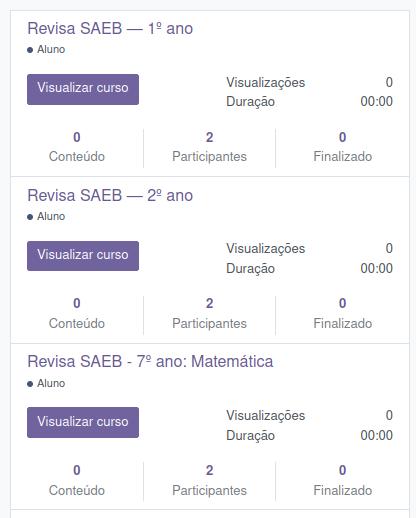
\includegraphics[width=.7\textwidth]{imgs/relatorio1}
\caption{Relatório para o coordenador ou professor}
\end{figure}

% André
% Explicar as seções, a relação com o material impresso, os quiz


